\documentclass[
../../Software_Engineering_Summary.tex,
]
{subfiles}

\externaldocument[ext:]{../../Software_Engineering_Summary.tex}
% Set Graphics Path, so pictures load correctly
\graphicspath{{../../}}

\begin{document}
\section{Design Principles}
A good software should have certain standards it should fulfill. The quality of a software can be measured.

\begin{defbox}
    [Quality Assurance]
    To create software we should first create a quality assurance plan, which is integrated into the software development process.

    \begin{itemize}
        \item Constantly asses design quality (quantitative and qualitative characteristics)
        \item Apply time-tested desing principles where applicable
        \item Use tools and design techniques that help to achieve quality
        \item Use design patterns (designs used across multiple projects, problems, etc.)
        \item Systematically verify correctness \& performance
        \item Validate fulfillment of Requirements
    \end{itemize}
\end{defbox}

\subsection{Good Software}
\subsubsection*{What is good software?}
    \begin{itemize}
        \item Internal quality factors
        \begin{itemize}
            \item Perceivable only by computer professionals 
            \item White box view
            \item Code, databases, documentation, etc.
        \end{itemize}
        \item External quality factors
        \begin{itemize}
            \item Perceived by the customer / user
            \item Depend on internal quality factors
            \item Black box view
            \item UI, speed, ease of use, etc.
        \end{itemize}
    \end{itemize}

\begin{defbox}
    [Internal quality factors]
    \begin{itemize}
        \item \textbf{Modularity:} How easy is it to modify the software?
        \item \textbf{Comprehensibility:} Is the software easy to understand?
        \item \textbf{Cohesion:} Is it clear what each component does?
        \item \textbf{Concision:} How concise is the code? (Code duplication, overly lengthy code)
        \item \textbf{Correctness:} Does the software work as intended?
    \end{itemize}
\end{defbox}

\begin{defbox}
    [External quality factors]
    \begin{itemize}
        \item \textbf{Validity:} Does the software work as according to the requirements?
        \begin{itemize}
            \item Needs precise requirements
            \item Depends on correct design
            \item Often conditional / codependant on correctness of internal quality factors
        \end{itemize}
        \item \textbf{Robustness:} How well does the software handle abnormal conditions and errors?
        \item \textbf{Extensibility:} Can the software be extended to fulfill new requirements?
        \begin{itemize}
            \item Architecture must be flexible / extensible
            \item Often dependant on modularity of internal quality factors
        \end{itemize}
        \item \textbf{Reusability:} How well can the software be reused in different contexts?
        \item \textbf{Compatibility:} How well does the software work with other software?
        \item \textbf{Portability:} How well does the software work on different platforms (hardware \& software)?
        \item \textbf{Efficiency:} How fast and resource-efficient is the software?
        \begin{itemize}
            \item Often depends on algorithms and data structures
            \item Should be implemented for the common case
        \end{itemize}
        \item \textbf{Usability:} How easy is it to use the software?
        \item \textbf{Functionality:} How far does the software usage extend?
        \begin{itemize}
            \item Features should be consistent in usage and design
        \end{itemize}
    \end{itemize}
\end{defbox}

Overall the most important quality factors of good software are:
\begin{itemize}
    \item \textbf{Maintainability:} Can be adjusted over time to new requirements
    \item \textbf{Efficiency:} Is reasonably fast and resource-efficient
    \item \textbf{Usability:} Is relatively easy to use and responsive
    \item \textbf{Dependability:} Does not cause physical or economical damage in case of system failure
\end{itemize}

\subsection{Measuring Software Quality}
In general, there are no universal way to measure quality as different software varies wildly. Oftentimes some metrics need to be negelected in favor of others, depending on the context (Usability over Security, Modularity over Concision, etc.).

What can be done is to define standards / heuristics to indicate quality of code. These are usually called \textbf{software metrics} or \textbf{code metrics}.

\begin{minipage}
    [t]{0.47\textwidth}
    \begin{defbox}
        [Software Metrics Pros]
        \begin{itemize}
            \item Can be computed mechanically
            \item Can be used to indicate bad design
        \end{itemize}
    \end{defbox}
\end{minipage}
\hfill
\begin{minipage}
    [t]{0.47\textwidth}
    \begin{defbox}
        [Software Metrics Cons]
        \begin{itemize}
            \item Does not take semantics into account
            \item False sense of correctness
        \end{itemize}
    \end{defbox}
\end{minipage}

\begin{defbox}
    [Code Metrics]
    \begin{itemize}
        \item \textbf{Fan-in / Fan-out:} 
        \begin{itemize}
            \item Fan-in: Number of functions that call a specific function
            \item Fan-out: Number of functions that are called by a specific function
        \end{itemize}
        \item \textbf{Length of code:} Number of lines of code, indicates complexity
        \item \textbf{Cyclomatic complexity:} Number of decision points in code (control-flow graph)
        \item \textbf{Depth of conditional nesting:} Number of nested conditional statements, hard to understand, hard to test
        \item \textbf{Weighted methods per class:} How many functions are in a class, functions are weighted dependend on size / complexity
        \item \textbf{Depth of Inheritance:} Number of levels of inheritance, hard to understand
    \end{itemize}
\end{defbox}

\subsubsection{Control-Flow Graph (CFG)}
A CFG represents all execution sequences of a program.

\begin{defbox}
    [Basic Blocks in a CFG]
    A basic block is a maximal sequence of non-branching statements or instructions that are always executed together.

    The execution of a basic block starts with the first statement, only the final statement can be a jump (branch or return).

    \begin{center}
        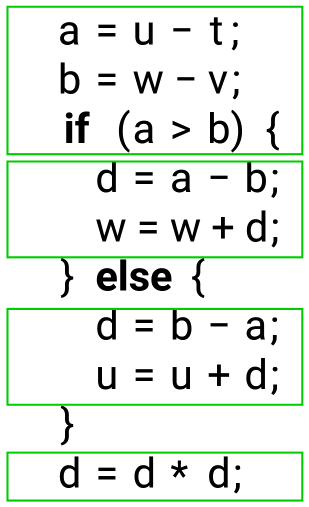
\includegraphics[height=110pt]{Pics/06/BasicBlocksCFG.png}
    \end{center}
\end{defbox}

\begin{defbox}
    [Control-Flow Graph]
    A Control-Flow Graph CFG(P) = (N, E, Label) of program P is a labeled directed graph, with nodes n $\in$ N which represent the basic blocks of P and edges e $\in$ E which represent the control flow of P. 
    Hereby each edge e = ($n_i$, lb, $n_j$) $\in$ E with $n_i$, $n_j$ $\in$ N and lb $\in$ Label is a transition from $n_i$ to $n_j$ with label lb.
    The labels represent the branching condition (Empty for returns and jumps).

    \begin{minipage}
        [t]{0.25\textwidth}
        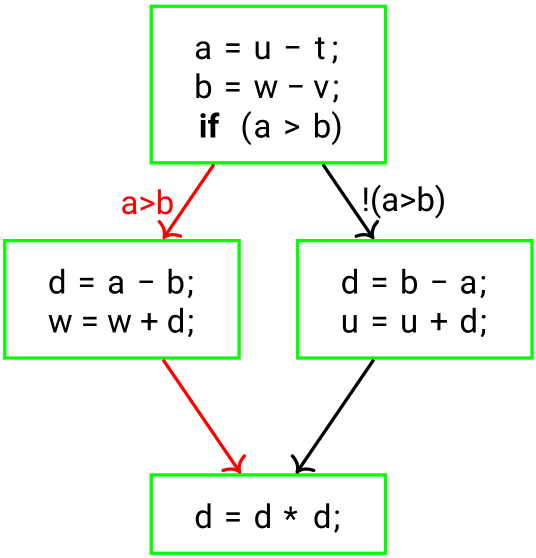
\includegraphics[height=120pt]{Pics/06/ExampleCFG.png}
        \captionof*{figure}{Red represents one possible execution sequence}
    \end{minipage}
    \hfill
    \begin{minipage}
        [t]{0.25\textwidth}
        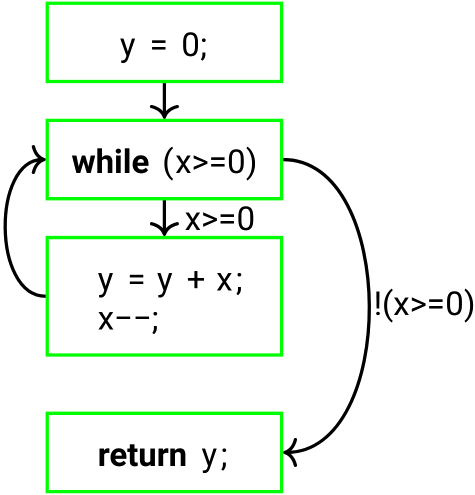
\includegraphics[height=120pt]{Pics/06/ExampleCFGLoop.png}
    \end{minipage}
    \hfill
    \begin{minipage}
        [t]{0.48\textwidth}
        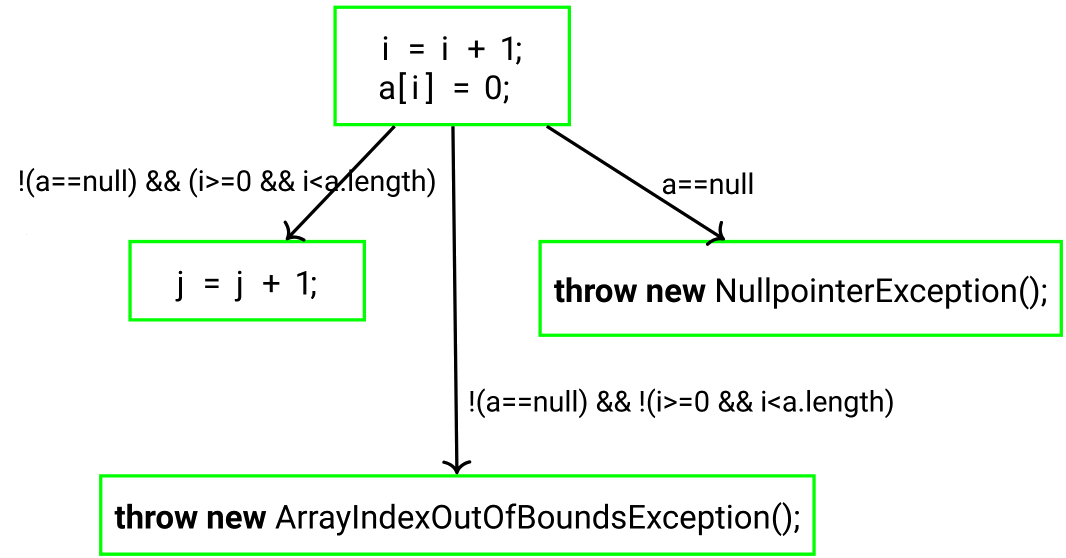
\includegraphics[height=120pt]{Pics/06/ExampleCFGExceptions.png}
    \end{minipage}
\end{defbox}

In many cases the definition of explicit initial and exit nodes is important.

\begin{figure}[htp]
    \begin{minipage}
        [t]{0.47\textwidth}
        \centering
        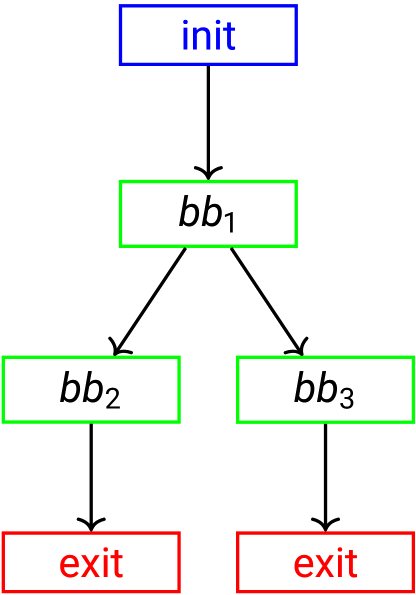
\includegraphics[height=120pt]{Pics/06/ExampleCFGInitialExit.png}
    \end{minipage}
    \hfill
    \begin{minipage}
        [t]{0.47\textwidth}
        \centering
        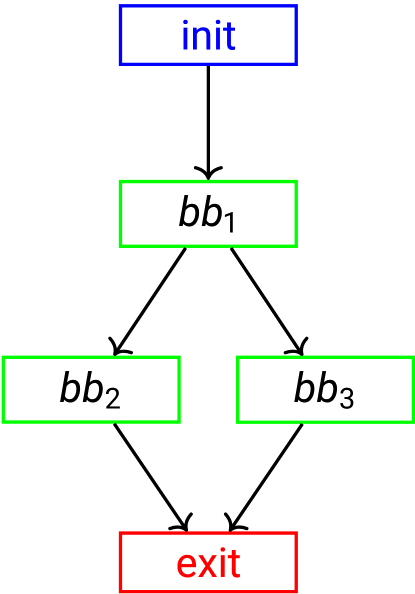
\includegraphics[height=120pt]{Pics/06/ExampleCFGSingleExit.png}
    \end{minipage}
\end{figure}

As there might be different end states sometimes the different exit nodes are important. For other reasons, like code metric computation, sometimes the exit nodes should be handled as a single node.

Sometimes code can result in unreachable nodes in one specific execution sequence. In this case the unreachable node / inactive edge should not be displayed.

\begin{figure}
    [htp]
    \centering
    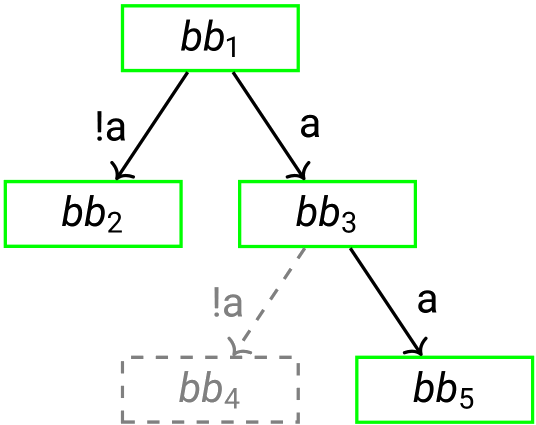
\includegraphics[height=120pt]{Pics/06/ExampleCFGInactiveEdges.png}
    \caption{Assumes $bb_3$ does not modify a}
\end{figure}

\subsubsection{Code Metric: Cyclomatic Complexity}
The cyclomatic complexity defines the number of independent paths through the code. It requires a CFG with a single exit node.
\begin{figure}
    [htp]
    \centering
    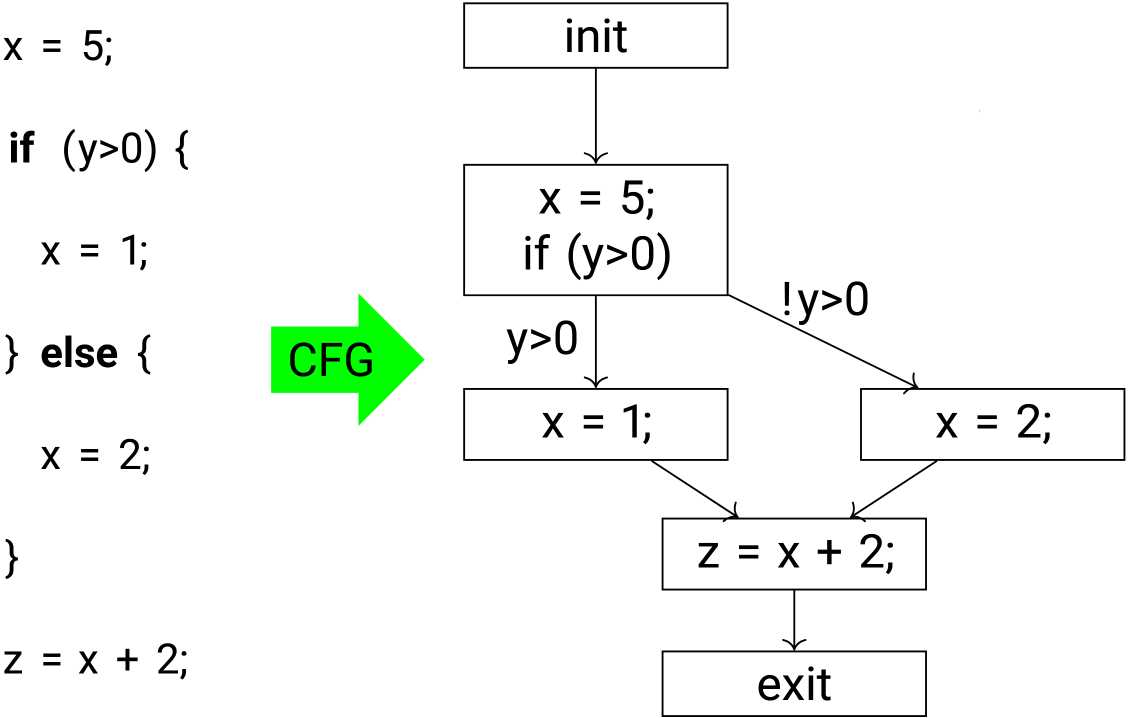
\includegraphics[scale=0.35]{Pics/06/CFGCyclomaticComplexity.png}
\end{figure}

Hereby the number of independent paths through the code is 2. This can be calculated like follows:


\begin{center}
    \begin{smallmathbox*}
        \shortstack{
            $C:= E - N + 2P$\\
            with $E$ edges, $N$ nodes and $P$ connected components
        }
    \end{smallmathbox*}
\end{center}

So in this example it would be:
\begin{center}
    \begin{smallmathbox*}
        $C = 6 - 6 + 2 * 1 = 2$
    \end{smallmathbox*}
\end{center}

In general, a cyclomatic complexit C of 10 or higher is considered to be complex - Rethinking design and coding might be beneficial.

\subsubsection{Code Metric: Class and Interface Coupling}
A class or interface C is coupled to a class or interface D if C requires D directly or indirectly.
Hereby a class or interface that depends on 2 classes is considered looser than one that depends on 8 classes.



\begin{defbox}
    [Common types of Coupling in OOP]
    \begin{itemize}
        \item Attribute referal: X has an attribute of Y
        \begin{itemize}
            \item \inlcodebox{class X \{ Y y; \}}
        \end{itemize}
        \item Expression referal: X contains an expression of Y
        \begin{itemize}
            \item \inlcodebox{class X \{ Object o = new Y(); \}}
            \item \inlcodebox{class X \{ void m() \{ \dots if (o instanceof Y) \dots \} \}}
        \end{itemize}
        \item Method referal: X calls a method of Y
        \begin{itemize}
            \item \inlcodebox{class X \{ void m() \{ \dots y.m(); \dots \} \}} (Object method)
            \item \inlcodebox{class X \{ void m() \{ \dots Y.m(); \dots \} \}} (Static method) 
        \end{itemize}
        \item Method-Instance referal: X has a method that references an instance of Y
        \begin{itemize}
            \item \inlcodebox{class X \{ X(Y y) \{ \dots \} \}} (Parameter)
            \item \inlcodebox{class X \{ Y f() \{ \dots \} \}} (Return type)
            \item \inlcodebox{class X \{ void m() \{ Y y = \dots; \} \}} (Local variable)
            \item \inlcodebox{class X \{ void m() \{ Object o = new Y(); \} \}} (Local Expression)
        \end{itemize}
        \item Inheritance: X inherits from Y
        \begin{itemize}
            \item \inlcodebox{class X extends Y \{ \dots \}} (Extension)
            \item \inlcodebox{class X implements Y \{ \dots \}} (Implementation)
        \end{itemize}
    \end{itemize}
\end{defbox}

\begin{defbox}
    [Design Principles: Tight and Loose Coupling]
    Tight coupling is generally undesirable
    \begin{itemize}
        \item Changes in couples classes may cause undesired changes in other classes
        \item Tight coupling makes it hard to understand a class in isolation
        \item Tight coupling makes it hard to reuse a class
        \item Tight coupling results in low modularity
    \end{itemize}

    Generic classes with high reusability must have very loose coupling. However, very loose coupling or no coupling in general is also undesirable.

    \begin{itemize}
        \item Goes aginst OOP principles
        \item Loose coupling may require a huge number of active objects, decreasing performance
    \end{itemize}

    However, the tightness of couplings needs to be determined on a case-by-case basis.
\end{defbox}

\subsubsection{Code Metric: Cohesion}
Cohesion measures the strength of the relation among elements of a class. All operations and data in a class should "naturally" belong to the concept modelled by the class. 

\begin{defbox}
    [Types of Cohesion]
    Ordered from undesirable to ideal:
    \begin{itemize}
        \item \defc{Coincidental}: No meaningful relation among elements
        \item \defc{Temporal}: Class elements are executed together
        \item \defc{Sequential}: Result of one method in input of another
        \item \defc{Communicational}: All functions access the same input or output
        \item \defc{Functional}: All elements contribute to achieve a single, well-defined purpose: \defc{Ideal} 
    \end{itemize}
\end{defbox}


\begin{defbox}
    [Lack of Cohesion of Methods (LCOM)]
    Cohesion is often evaluated by the \defc{Lack of Cohesion of Methods (LCOM)} metric.
    Hereby, a class C is defined as a set of instance fields F and methods M (excluding constructors). 
    This set is then used to define an undirected Graph G(M,E) with vertices M and Edges E.
    
    \begin{center}
        \begin{smallmathbox*}
            $E = \{\langle m_1, m_2\rangle \in M \times M | \exists f \in F : m_1 \text{ and } m_2 \text{ access } f, m_1 \not = m_2\}$
        \end{smallmathbox*}
    \end{center}
    The LCOM(C) is then defined as the number of \defc{connected components (CC)} of G(M,E). 
    This means that for a class C with |M| = n, the LCOM(C) $\in [0, n]$. Therefore a high LCOM value indicates low cohesion.

    An issue with this metric is that its definition needs to be refined for special methods, like the constructors, hashCode, toString etc. methods. While these are technically part of the class, they are considered standard components of each class and therefore do not count towards the LCOM.
\end{defbox}

Low Cohesion is generally undesirable. As the classes can be hard to comprehend, reuse and maintain. Low cohesion also often indicates too-corse abstraction, meaning classes take responsibility for too many tasks, that should be handled by other classes.

As a rule of thumb: A class with high cohesion can often be described in a single sentence.
\end{document}